\documentclass{article}
\usepackage[utf8]{inputenc}
\usepackage{polski}
\usepackage{graphicx}
\usepackage{fancyhdr}
\usepackage{lastpage}
\usepackage{listings}


\pagestyle{fancy}

\fancyhf{}

\fancyfoot[C]{\thepage\ / \pageref{LastPage}} % Ustawienie numeracji stron w stopce

\fancypagestyle{plain}{ % Nadpisanie stylu strony tytułowej
    \fancyhf{}
    \renewcommand{\headrulewidth}{0pt} % Usunięcie nagłówka
    \fancyfoot[C]{\thepage\ / \pageref{LastPage}}
}

\title{Specyfikacja funkcjonalna projektu 2 w języku Java}
\author{Miłosz Mertka i Sebastian Grosfeld}
\date{\today}

\begin{document}

\maketitle

\tableofcontents

\newpage

% Poniżej ustawiany jest nagłówek
\setlength{\headheight}{23pt}
\lhead{Miłosz Mertka\\Sebastian Grosfeld}
\rhead{Specyfikacja funkcjonalna\\ projektu 2 w języku Java}

\section{Wstęp teoretyczny}

Program porusza zagadnienia teorii grafów. Teoria grafów to dziedzina informatyki zajmująca się badaniem zjawisk przy wykorzystaniu grafów. Graf definiuje się następująco: $G=(V,E)$. $V$ jest zbiorem wierzchołków grafu, $E$ jest zbiorem jego krawędzi. \emph{Rysunek \ref{fig:graph}} pokazuje przykładowy graf.

\begin{figure}[htp]
    \centering
    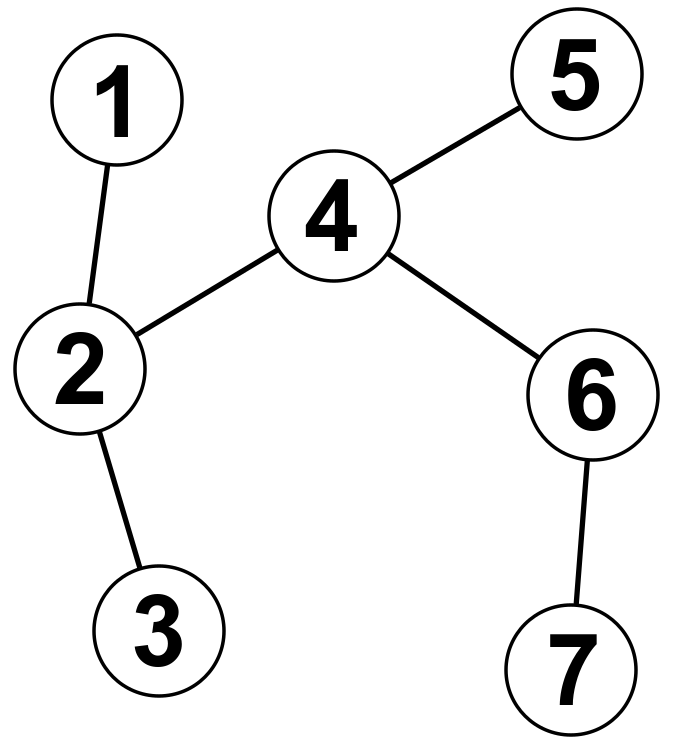
\includegraphics[width=5cm]{images/graph.png}
    \caption{Przykładowy graf}
    \label{fig:graph}
\end{figure}

Grafy można podzielić na \emph{nieskierowane} i \emph{skierowane}. Te pierwsze posiadają drogę zarówno z wierzchołka A do wierzchołka B, ale także z wierzchołka B\linebreak do wierzchołka A. Grafy skierowane natomiast nie muszą posiadać zdefiniowanych przejść w obie strony dla danej pary wierzchołków A i B. W grafach skierowanych wierzchołki są ze sobą połączone łukami, które wskazują kierunek przejścia z jednego wierzchołka do drugiego (\emph{Rysunek \ref{fig:directed_graph}}).

\begin{figure}[htp]
    \centering
    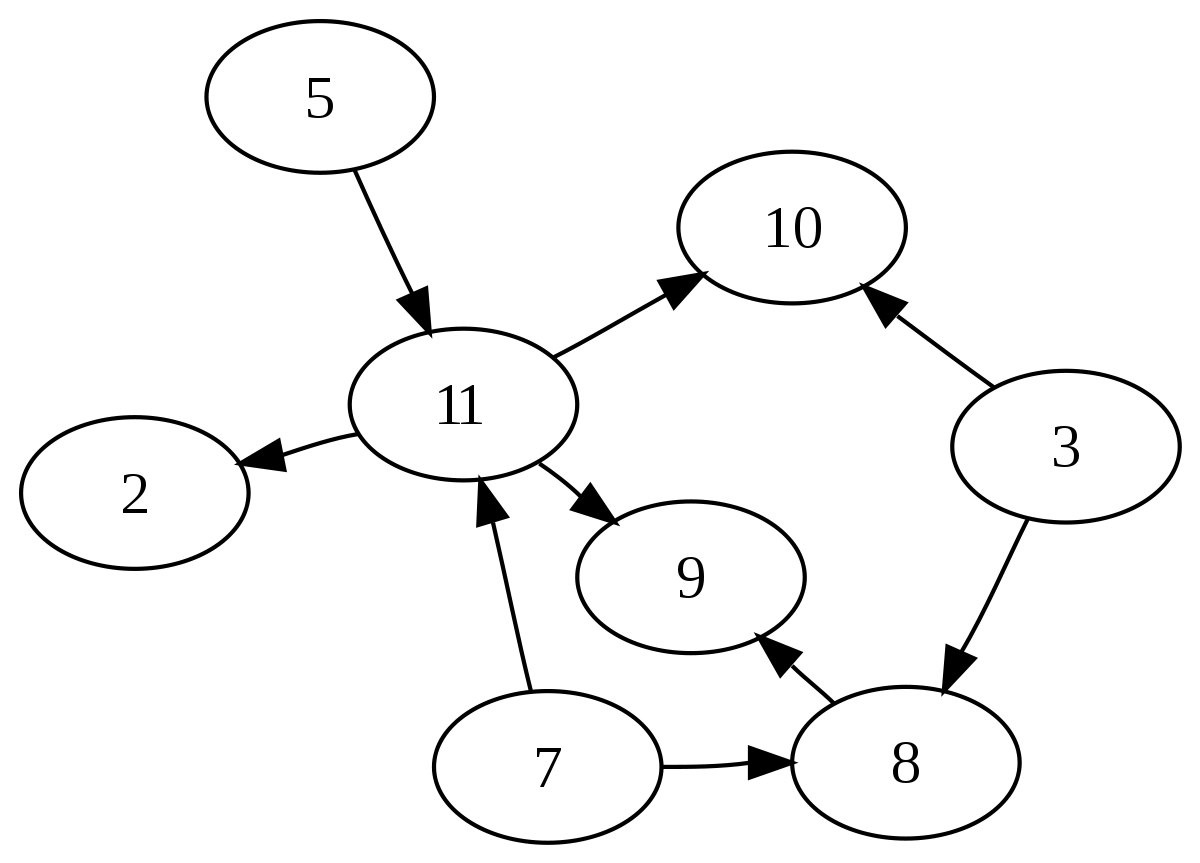
\includegraphics[width=7cm]{images/directed_graph.png}
    \caption{Przykładowy graf skierowany}
    \label{fig:directed_graph}
\end{figure}

\newpage
Krawędzie w grafach mogą również posiadać różne wagi. Taki graf nazywa się \emph{grafem ważonym}. Waga określa koszt przejścia z jednego wierzchołka\linebreak do drugiego. Przykładowy graf ważony przedstawia \emph{Rysunek \ref{fig:weight_graph}}. W przypadku grafu skierowanego można zdefiniować różne wagi dla dwóch łuków łączących tą samą parę wierchołków.

\begin{figure}[htp]
    \centering
    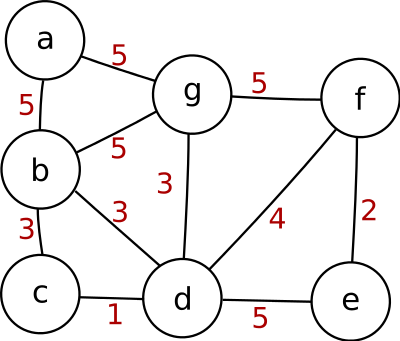
\includegraphics[width=6cm]{images/graph_weights.png}
    \caption{Przykładowy graf nieskierowany ważony}
    \label{fig:weight_graph}
\end{figure}

Grafy bada się pod kątem ich \emph{spójności}. Graf jest spójny, jeśli zawsze istnieje droga między dowolnymi wierzchołkami grafu. Do badania spójności grafu można wykorzystać znane algorytmy przeszukiwania grafu. \emph{Rysunek \ref{fig:inconsistent_graph}} pokazuje przykładowy graf niespójny.

\begin{figure}[htp]
    \centering
    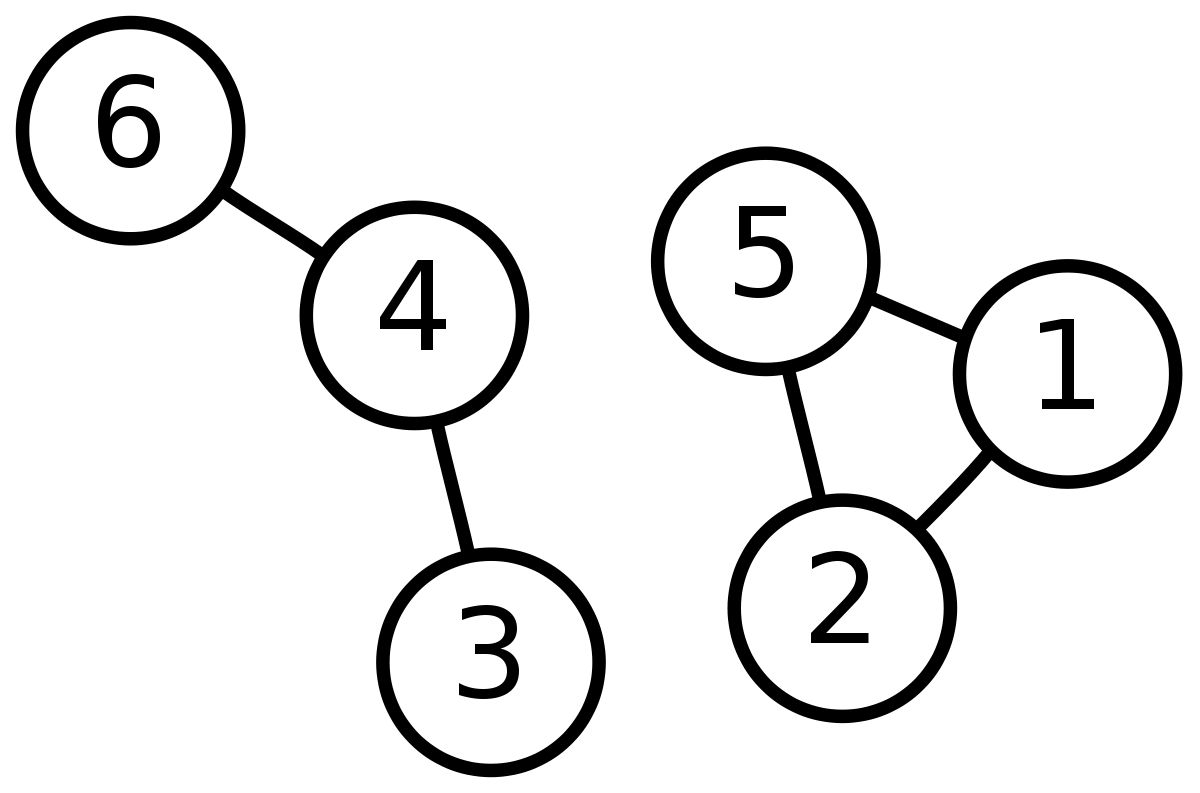
\includegraphics[width=5cm]{images/graph_inconsistent.png}
    \caption{Przykładowy graf niespójny}
    \label{fig:inconsistent_graph}
\end{figure}

Grafy posiadają praktyczne zastosowanie między innymi w systemach nawigacji drogowej. Tutaj za wierzchołki grafu można potraktować kolejne skrzyżowania, krawędzie to drogi łączące te skrzyżowania, a waga to koszt przejazdu\linebreak od jednego skrzyżowania do drugiego. W ten sposób można następnie zastosować znane algorytmy szukania optymalnej drogi w grafie między zadanymi wierzchołkami. W wyniku tego można otrzymać w nawigacji samochodowej optymalną trasę dojazdu do zadanego celu.

\section{Cel projektu}
Celem projektu jest stworzenie programu posiadającego interfejs graficzny,\linebreak który będzie w stanie wykonać następujące zadania:
\begin{enumerate}
    \item Wygeneruje graf w postaci siatki (\emph{Rysunek \ref{fig:graf_pp}}) o podanej ilości kolumn\linebreak i wierszy, wierzchołki i wagi krawędzi losowane w podanym zakresie wartości.
    \item Zapisze taki graf do pliku o ustalonym formacie.
    \item Przeczyta z pliku o ustalonym formacie taki graf.
    \item Potrafi określić czy dany graf jest spójny za pomocą algorytmu BFS.
    \item Potrafi wyznaczyć w tym grafie najkrótsze ścieżki pomiędzy wybranymi parami wierzchołków, korzystając z algorytmu Dijkstry.
\end{enumerate}

\begin{figure}[htp]
        \centering
        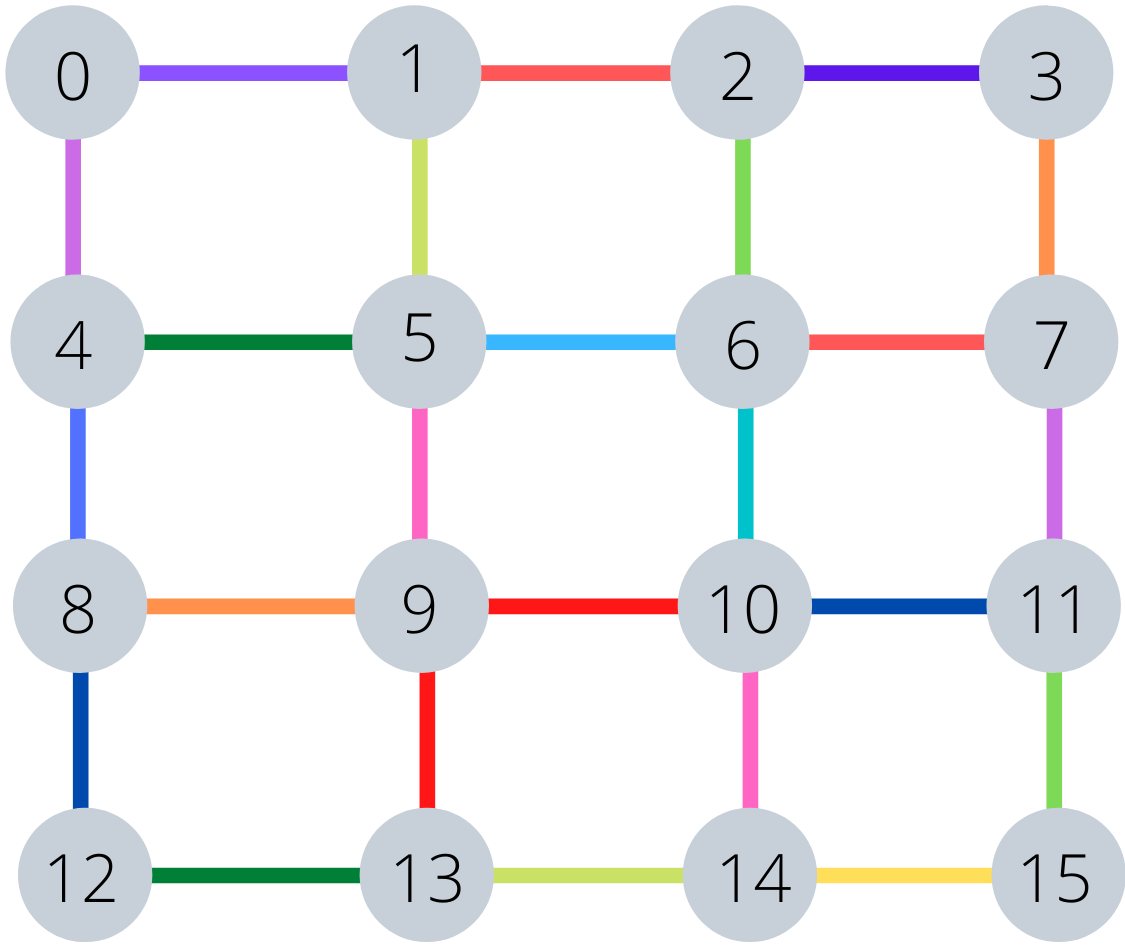
\includegraphics[width=5cm]{images/graf_pp.png}
        \caption{Wizualizacja przykładowego, wygenerowanego grafu}
        \label{fig:graf_pp}
\end{figure}

\newpage

\section{Obsługa programu}

\begin{figure}[htp]
        \centering
        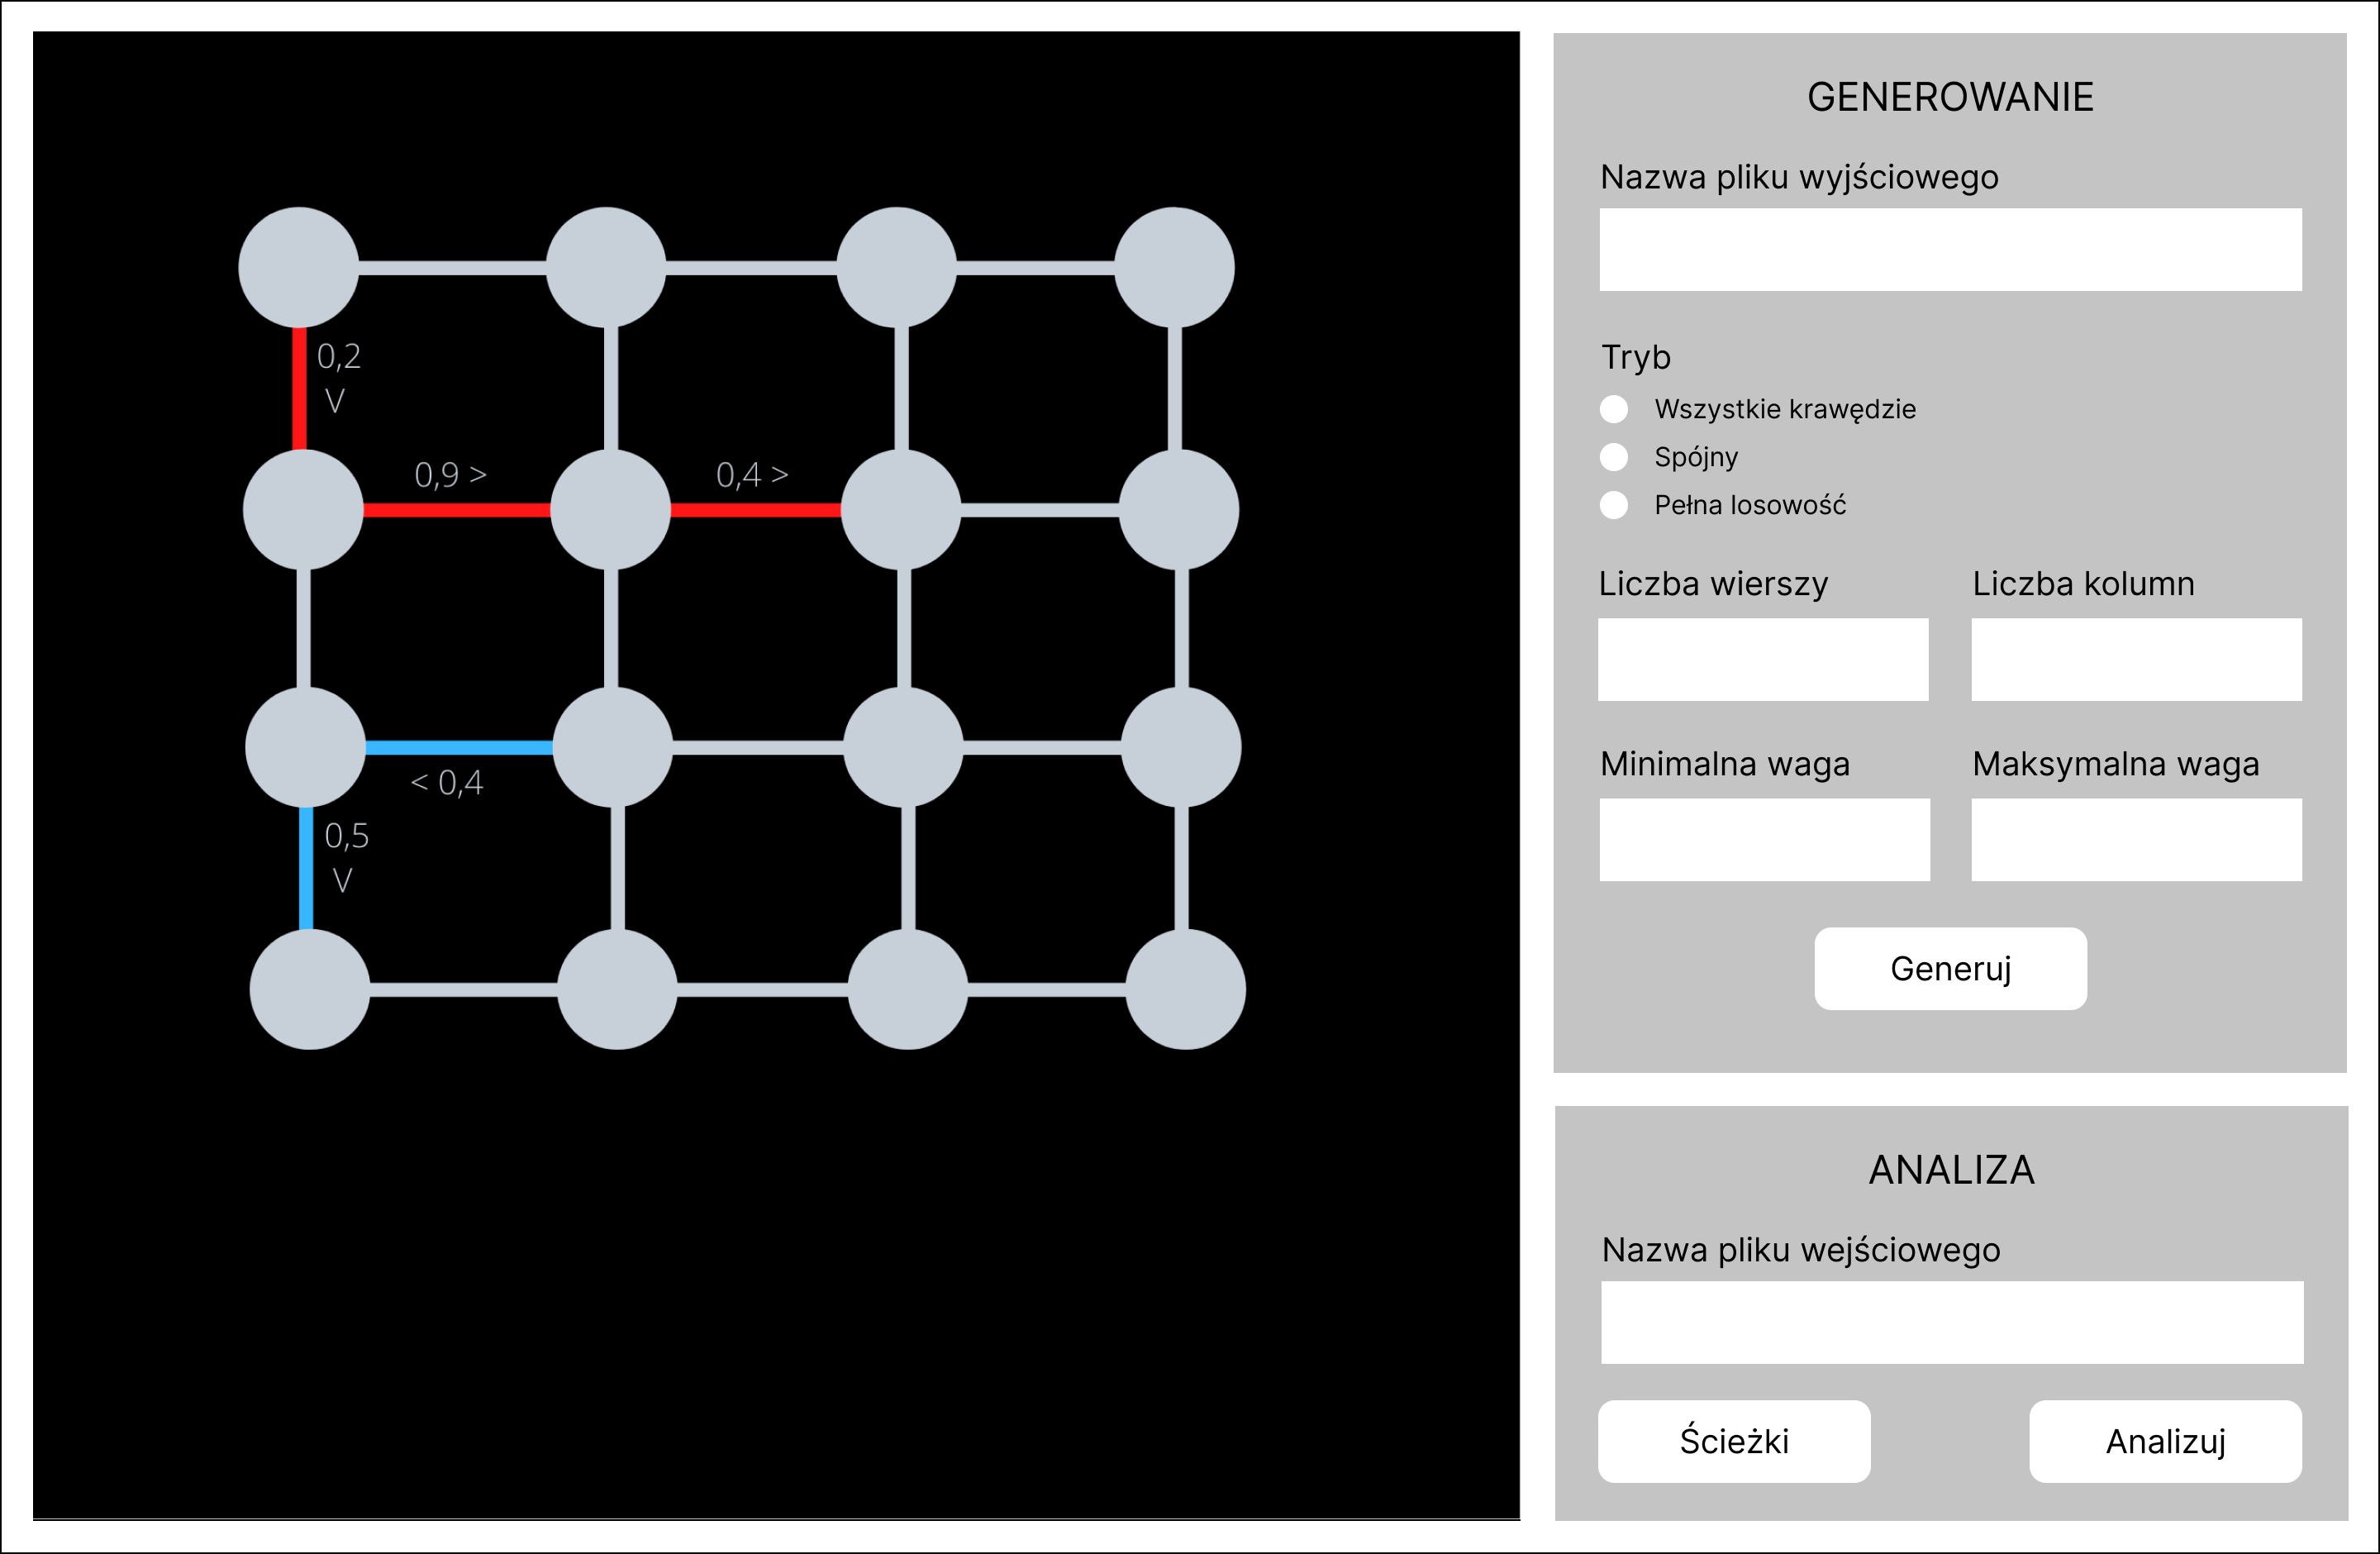
\includegraphics[width=13cm]{images/gui_main.png}
        \caption{Główne okno programu}
        \label{fig:gui_main}
\end{figure}
Program będzie skompilowany jako plik typu Jar. Uruchomienie go będzie odbywać się z linii poleceń przez wpisanie \textit{java -jar [ścieżka do pliku]}.
Program posiada tryb generujący graf i zapisujący go do pliku oraz analizujący graf zapisany w pliku. Aby skorzystać z pierwszego należy w polu \textbf{Nazwa pliku wyjściowego} wpisać nazwę pliku do którego chcemy zapisać wygenerowany graf. Następnie należy wybrać jeden z dostępnych trybów genreacji:

\begin{itemize}
    \item \textbf{Wszystkie krawędzie} -- wygenerowany graf posiada wszystkie krawędzie oraz wagi losowane z podanego przedziału.
    \item \textbf{Spójny} -- wygenerowany graf jest spójny (niekoniecznie musi posiadać wszystkie krawędzie) i posiada wagi zawierające się w podanym przedziale.
    \item \textbf{Pełna losowość} -- wygenerowany graf nie posiada gwaracji spójności,\linebreak a krawędzie losowane są z podangeo przedziału. 
\end{itemize}

Potem należy wypełnić pola \textbf{Liczba wierszy} i \textbf{Liczba kolumn} podając wymiary grafu oraz pola \textbf{Minimalna waga} i \textbf{Maksymalna waga} podając przedział losowania wag krawędzi. Na koniec trzeba kliknąć przycisk\linebreak \textbf{Generuj}. Jeśli podano prawidłowe dane to pownien wyświetlić się w głównym oknie programu wygenerowany graf.

\newpage

Aby skorzystać z trybu analizującego należy w polu \textbf{Nazwa pliku wejściowego} podać nazwę pliku zawierającego graf, który ma być poddany analizie\linebreak i kliknąć przycisk \textbf{Analizuj}. Zostanie wyświetlony komunikat o tym, czy dany graf jest spójny, a analizowany graf pojawi się w oknie głównym.
Następnie klikając przycisk \textbf{Ścieżki}, otworzy się okno konfiguracji ścieżek o nazwie \textbf{Szukanie najkrótszych ścieżek}. Będąc w nim możemy dodawać, ukrywać, usuwać ścieżki oraz wybierać dla nich początki i końce. Wpisane ścieżki pojawią się\linebreak na grafie. Mamy możliwość także pokazywania wag. Dodawać i zaznaczać ścieżki możemy też bezpośrednio na wyświetlanym grafie. Klikając raz lewym przyciskiem myszki na wierzchołek oznaczamy początek danej ścieżki, a klikając lewym przyciskiem myszki i jednoczeście trzymając wciśnięty klawisz \textbf{Shift} oznaczamy koniec danej ścieżki. Ścieżki zaznaczane są różnymi kolorami. Po zaznaczeniu ich na grafie (\emph{Rysunek \ref{fig:gui_main}}) ścieżki pojawią się w oknie \textbf{Szukanie najkrótszych ścieżek}.

Jeśli nie podamy pliku wejściowego do analizy, to rozważany będzie graf wcześniej wygenerowany za pomocą trybu generującego widoczny w oknie głównym. Pliki wejściowe i wyjściowe będą przechowywane w katalogu, w którym zlokalizowany jest program.

Aby zakończyć pracę z programem należy go zamknąć poprzez wciśnięcie symbolu \textbf{X} w prawym górnym rogu okna.

\begin{figure}[htp]
        \centering
        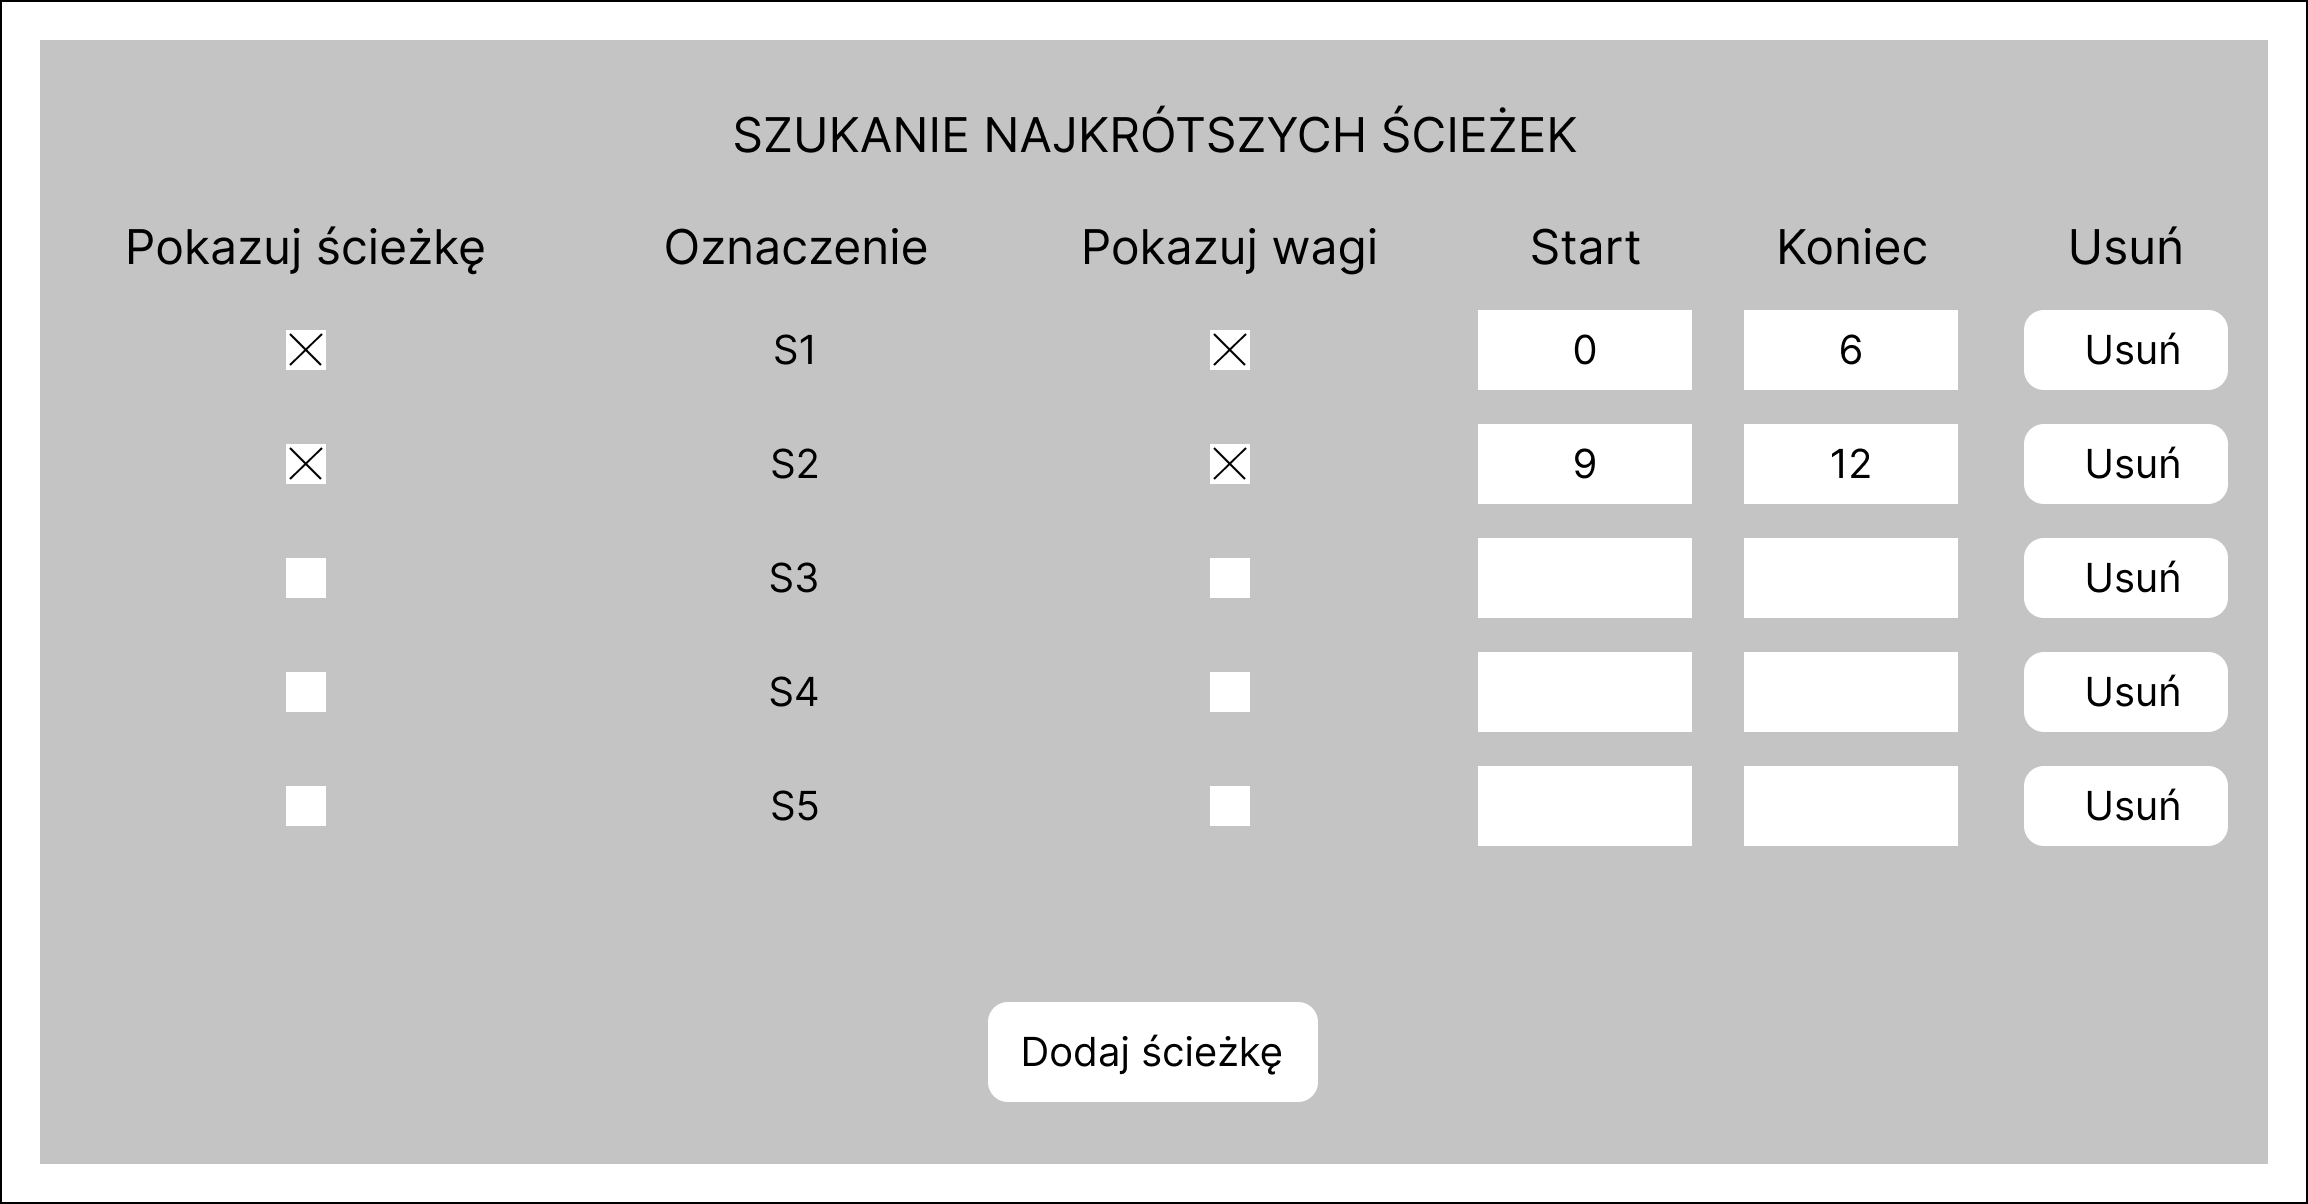
\includegraphics[width=13cm]{images/gui_paths.png}
        \caption{Okno konfiguracji ścieżek}
        \label{fig:gui_paths}
\end{figure}

\newpage

\section{Komunikaty błędów}
Wszystkie błędy wyświetlają się w formie alertu z odpowiednim komunikatem (\emph{Rysunek \ref{fig:gui_error}}).

\begin{figure}[htp]
        \centering
        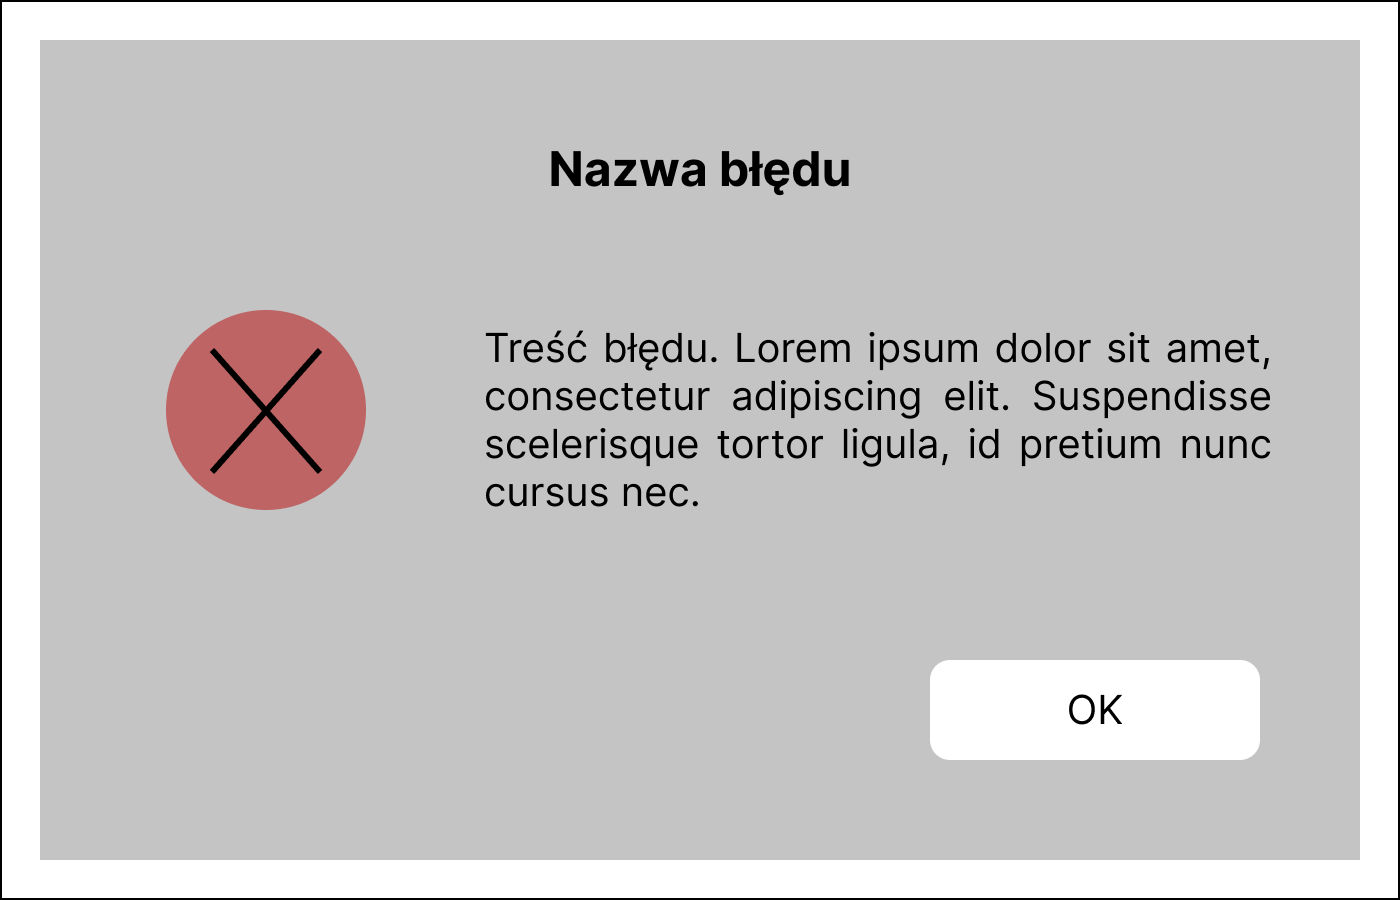
\includegraphics[width=8cm]{images/gui_error.png}
        \caption{Okno komunikatu o błędzie}
        \label{fig:gui_error}
\end{figure}

Możliwe komunikaty błędów:
\begin{itemize}
    \item \textbf{Błąd odczytu/zapisu pliku} -- nie udało się otworzyć pliku do odczytu lub zapisu.
    \item \textbf{Wagi nie mogą być ujemne} -- podane wartości wag są ujemne.
    \item \textbf{Minimalna waga nie może być większa od maksymalnej} -- podano większą wartość dla minimalnej wagi niż dla wagi maksymalnej.
    \item \textbf{Liczba wierszy musi być większa od 0} -- podano nieprawidłową liczbę wierszy.
    \item \textbf{Liczba kolumn musi być większa od 0} -- podano nieprawidłową liczbę kolumn.
    \item \textbf{Błędna konfiguracja ścieżek} -- podane wartości wierzchołków startowych i końcowych pochodzą spoza dziedziny (numery wierzchołków danego grafu) lub wierzchołek startowy jest taki sam jak końcowy.
\end{itemize}

\end{document}
